% Options for packages loaded elsewhere
\PassOptionsToPackage{unicode}{hyperref}
\PassOptionsToPackage{hyphens}{url}
%
\documentclass[
]{article}
\usepackage{lmodern}
\usepackage{amssymb,amsmath}
\usepackage{ifxetex,ifluatex}
\ifnum 0\ifxetex 1\fi\ifluatex 1\fi=0 % if pdftex
  \usepackage[T1]{fontenc}
  \usepackage[utf8]{inputenc}
  \usepackage{textcomp} % provide euro and other symbols
\else % if luatex or xetex
  \usepackage{unicode-math}
  \defaultfontfeatures{Scale=MatchLowercase}
  \defaultfontfeatures[\rmfamily]{Ligatures=TeX,Scale=1}
\fi
% Use upquote if available, for straight quotes in verbatim environments
\IfFileExists{upquote.sty}{\usepackage{upquote}}{}
\IfFileExists{microtype.sty}{% use microtype if available
  \usepackage[]{microtype}
  \UseMicrotypeSet[protrusion]{basicmath} % disable protrusion for tt fonts
}{}
\makeatletter
\@ifundefined{KOMAClassName}{% if non-KOMA class
  \IfFileExists{parskip.sty}{%
    \usepackage{parskip}
  }{% else
    \setlength{\parindent}{0pt}
    \setlength{\parskip}{6pt plus 2pt minus 1pt}}
}{% if KOMA class
  \KOMAoptions{parskip=half}}
\makeatother
\usepackage{xcolor}
\IfFileExists{xurl.sty}{\usepackage{xurl}}{} % add URL line breaks if available
\IfFileExists{bookmark.sty}{\usepackage{bookmark}}{\usepackage{hyperref}}
\hypersetup{
  pdftitle={COVID-19 modeling in South Dakota},
  hidelinks,
  pdfcreator={LaTeX via pandoc}}
\urlstyle{same} % disable monospaced font for URLs
\usepackage[margin=1in]{geometry}
\usepackage{longtable,booktabs}
% Correct order of tables after \paragraph or \subparagraph
\usepackage{etoolbox}
\makeatletter
\patchcmd\longtable{\par}{\if@noskipsec\mbox{}\fi\par}{}{}
\makeatother
% Allow footnotes in longtable head/foot
\IfFileExists{footnotehyper.sty}{\usepackage{footnotehyper}}{\usepackage{footnote}}
\makesavenoteenv{longtable}
\usepackage{graphicx,grffile}
\makeatletter
\def\maxwidth{\ifdim\Gin@nat@width>\linewidth\linewidth\else\Gin@nat@width\fi}
\def\maxheight{\ifdim\Gin@nat@height>\textheight\textheight\else\Gin@nat@height\fi}
\makeatother
% Scale images if necessary, so that they will not overflow the page
% margins by default, and it is still possible to overwrite the defaults
% using explicit options in \includegraphics[width, height, ...]{}
\setkeys{Gin}{width=\maxwidth,height=\maxheight,keepaspectratio}
% Set default figure placement to htbp
\makeatletter
\def\fps@figure{htbp}
\makeatother
\setlength{\emergencystretch}{3em} % prevent overfull lines
\providecommand{\tightlist}{%
  \setlength{\itemsep}{0pt}\setlength{\parskip}{0pt}}
\setcounter{secnumdepth}{-\maxdimen} % remove section numbering
\usepackage{booktabs}
\usepackage{longtable}
\usepackage{array}
\usepackage{multirow}
\usepackage{wrapfig}
\usepackage{float}
\usepackage{colortbl}
\usepackage{pdflscape}
\usepackage{tabu}
\usepackage{threeparttable}
\usepackage{threeparttablex}
\usepackage[normalem]{ulem}
\usepackage{makecell}
\usepackage{xcolor}

\title{COVID-19 modeling in South Dakota}
\author{}
\date{\vspace{-2.5em}April 2020}

\begin{document}
\maketitle

\hypertarget{authors}{%
\section{Authors}\label{authors}}

\emph{Jeff Wesner, Ph.D.}\textsuperscript{1}, \emph{Dan Van Peursem,
Ph.D.}\textsuperscript{2}, \emph{Jose Flores,
Ph.D.}\textsuperscript{2,3}, \emph{Yuhlong Lio,
Ph.D.}\textsuperscript{2}

University of South Dakota

\textsuperscript{1}Department of Biology, \textsuperscript{2}Department
of Mathematical Sciences, \textsuperscript{3}Department of Computer
Science

\href{mailto:Jeff.Wesner@usd.edu}{\nolinkurl{Jeff.Wesner@usd.edu}}

\hypertarget{purpose}{%
\section{Purpose}\label{purpose}}

To predict hospital bed needs, ICU needs, and ventilator needs in South
Dakota due to COVID-19.

\hypertarget{general-approach-and-justification}{%
\section{General Approach and
Justification}\label{general-approach-and-justification}}

We estimated R0 from current incidence rates in South Dakota. We then
fit SIR models using our estimates of R0 and compared model predictions
to actual values of hospitalizations reported by the South Dakota
Department of Health (data source:
\url{https://www.keloland.com/keloland-com-original/why-south-dakotas-number-of-deaths-isnt-always-up-to-date/}.
We chose this approach because it does not rely on external estimates of
R0, but instead derives them from data specific to South Dakota.

Because our estimates of R0 are derived from reported incidence data,
they reflect any day-to-day adjustments in R0 due to social distancing
(with an unknown lag time). In other words, as social distancing reduces
incidence, that will be reflected in our estimates of R0. It is worth
noting that reported incidence is almost certainly lower than true
incidence. However, this does not alter our estimates of R0, assuming
that the rate of underreporting is constant across time.

\hypertarget{derivation-of-r0}{%
\section{Derivation of R0}\label{derivation-of-r0}}

We used the following equation to estimate R0 (eqn 3.1 in Wallinga and
Lipsitch 2007)
\url{https://www.ncbi.nlm.nih.gov/pmc/articles/PMC1766383/?report=reader\#!po=83.3333}:

\[R0 = 1 + r/b\]

where 1/b is the generation time (aka serial interval) in days, and
\emph{r} is the slope of a linear regression between daily incidence and
time. This approach is recommended during the initial phase of an
epidemice when growth is approximately log-linear.

We estimated a posterior distribution of \emph{r} using reported
incidence data in the following regression:

\[log(y_i) \sim N(\mu_i, \sigma)\] \[\mu_i = \alpha + \beta x_i\]
\[\alpha \sim N(0,1)\] \[\beta \sim N(0,1)\]
\[\sigma \sim HalfCauchy(0,1)\] where \emph{log}(\(y_i\)) is
log-transformed incidence on date \(i\), distributed as a normal
distribution with a mean \(\mu_i\) and standard deviation \(\sigma\),
\(\alpha\) is the intercept, \(\beta\) is the slope (aka \emph{r}).The
prior distributions for each parameter are below the regression
equation.

The outcome of that regression is below. It shows a clear dip in
incidence over the last 3-4 days, though this has had a minimal effect
thus far on our estimates of \emph{r}. More importantly, our main
comparison to model fit is the number of cumulative hospitalizations,
which continue to track the model predictions (scroll below for the
graph).

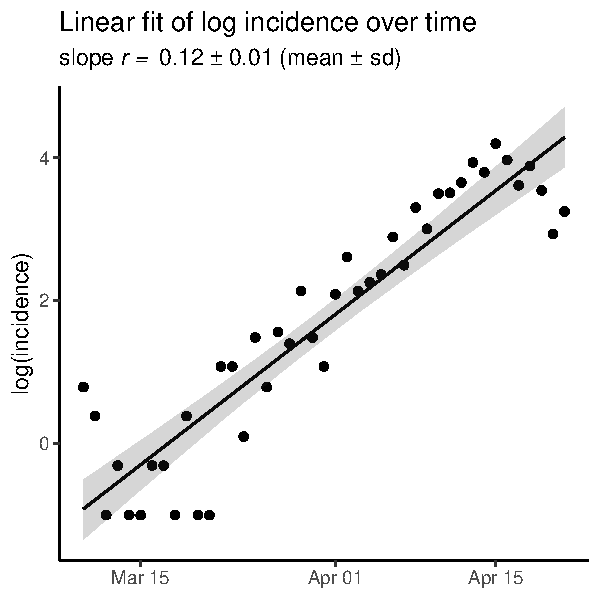
\includegraphics{script_SIR_sims_publish_files/figure-latex/unnamed-chunk-4-1.pdf}

We simulated uncertainty in R0 by sampling from the posterior
distribution of \emph{r} 500 times and re-calculating the equation for
R0 each time. We did this under three scenarios of generation time (4,
6, or 7 days). These were chosen based on Park et al.~(2020) who
estimated a generation time for COVID-19 of 4-8 days -
\url{https://www.mdpi.com/2077-0383/9/4/967}. The table below shows the
estimated R0 under three assumptions of generation time. Five hundred
samples from these values were entered into the following SIR model:

\begin{longtable}[]{@{}lrr@{}}
\caption{Table 1. R0 values and generation times (days) used to fit the
SIR model.}\tabularnewline
\toprule
generation\_time & mean & sd\tabularnewline
\midrule
\endfirsthead
\toprule
generation\_time & mean & sd\tabularnewline
\midrule
\endhead
GT4 & 1.49 & 0.03\tabularnewline
GT6 & 1.74 & 0.05\tabularnewline
GT7 & 1.87 & 0.06\tabularnewline
\bottomrule
\end{longtable}

\[\frac{dS}{dt} = \frac{\beta*S*I}N\]

\[\frac{dI}{dt} = \frac{\beta*S*I}N - \gamma*I\]

\[\frac{dR}{dt} = \gamma*I\]

where \(\gamma\) is 1/\(days_{infected}\), \(\beta\) is \(gamma\)*R0,
\(days_{infected}\) is 7, and \(N\) is \(S+I+R\). We simulated 200 days
of infection and assumed starting values for S = 0.99999, I = 0.000001,
and R = 0.000009.

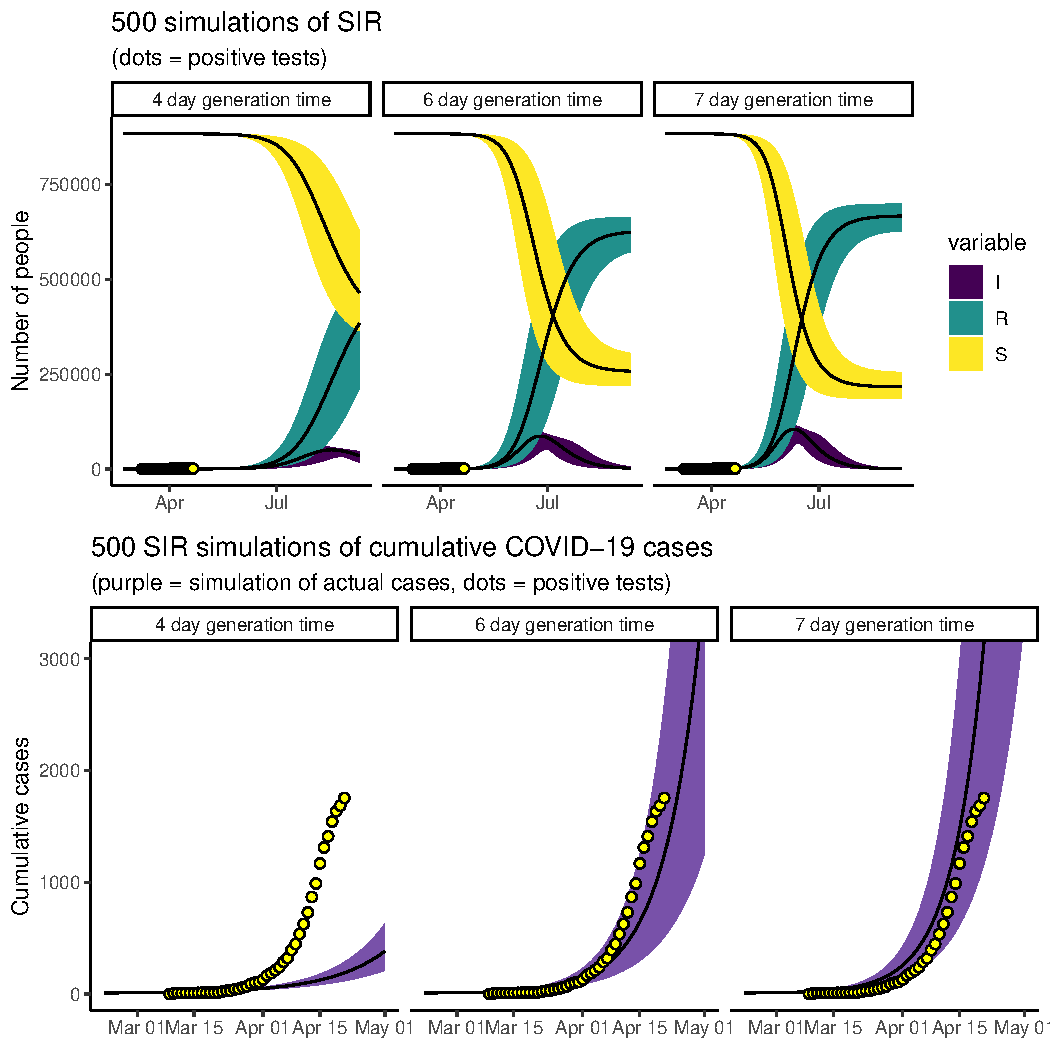
\includegraphics{script_SIR_sims_publish_files/figure-latex/unnamed-chunk-7-1.pdf}
The graphs above show the outcome of the SIR model under 4, 6, or 7 day
generation times. Lines are the mean predictions, shaded areas are the
2.5 and 97.5\% quantiles, and the dots are the reported data from SD
DOH.

\#Hospital Beds, ICU beds, and Ventilators From the predictions of cases
above, we estimated the number of hospital beds, ICU beds, and
ventilators needed by assuming that 4\% of cases would need
hospitalization, 1.5\% of cases would need an ICU bed, and 1.05\% of
cases would need a ventilator. We also assumed a mean stays in the
hospital system as a whole of 7, 8, or 10 days for hospitalization, ICU,
and ventilator, respectively.

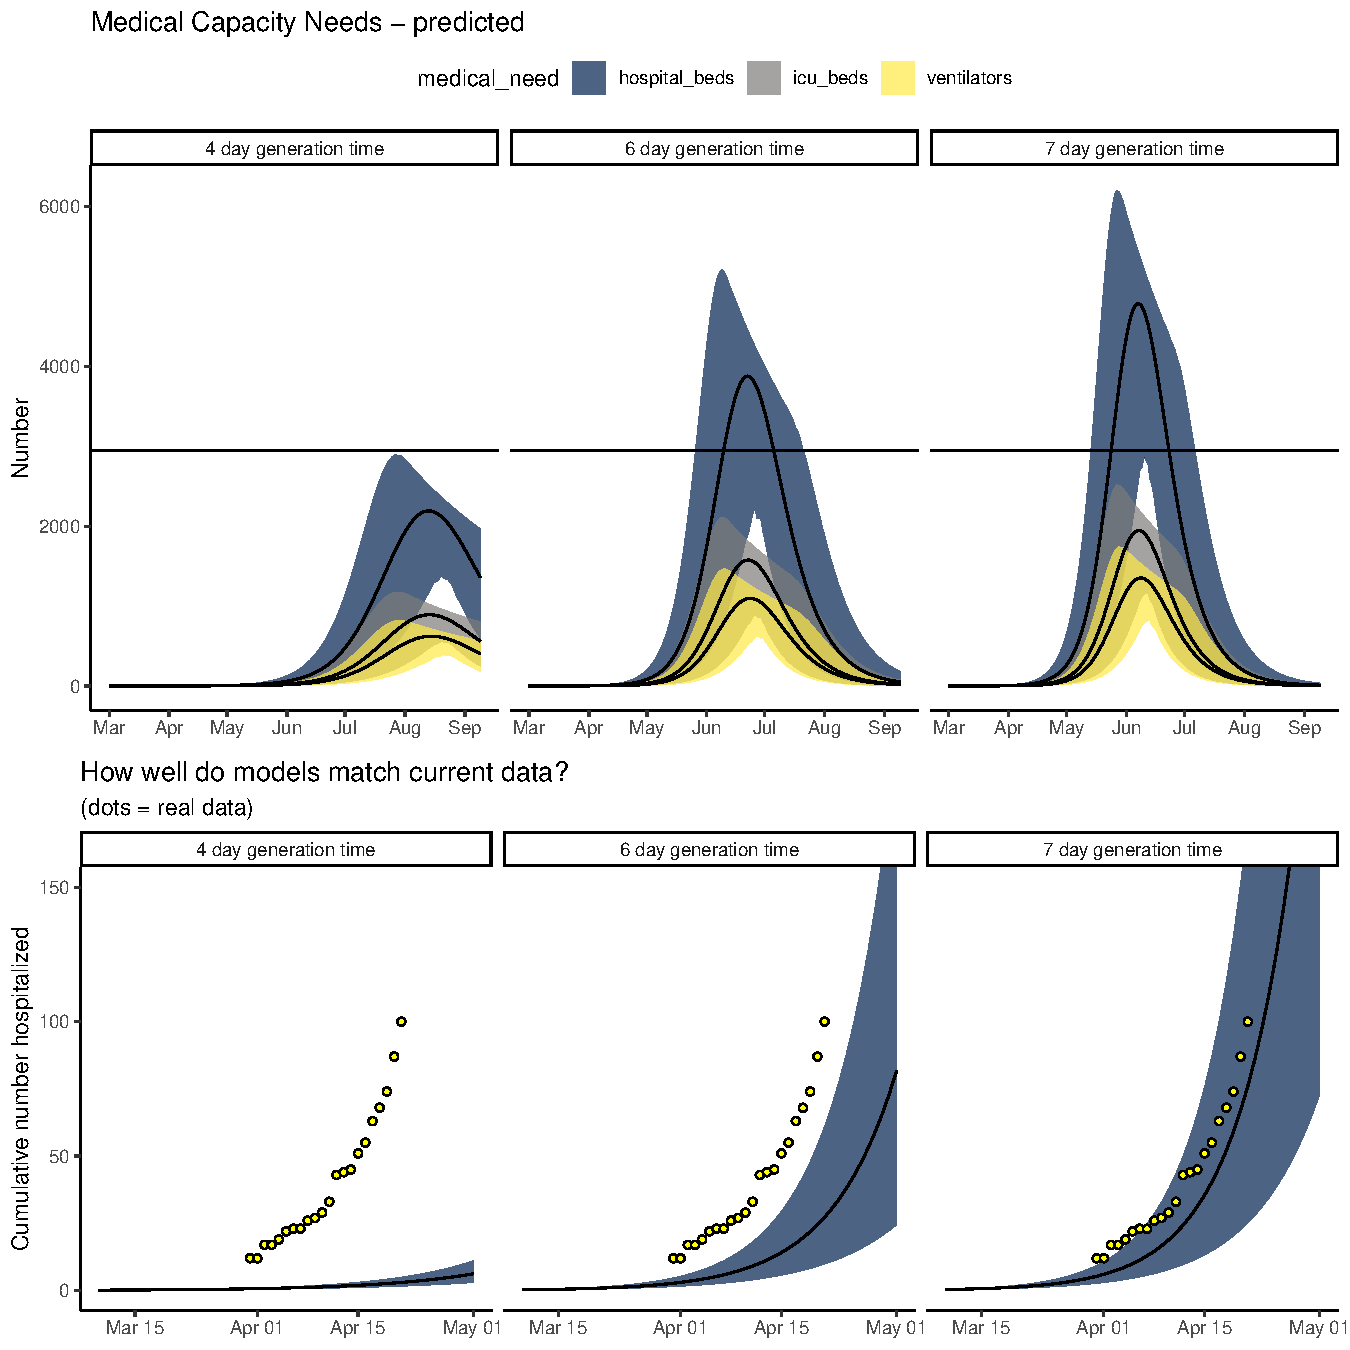
\includegraphics{script_SIR_sims_publish_files/figure-latex/unnamed-chunk-8-1.pdf}

This plot shows the predicted number of hospital beds, ICU beds, and
ventilators needed under each scenario. The horizontal black line shows
the total number of hospital beds in South Dakota*.

The plot on the bottom shows the predicted \emph{cumulative} number of
beds compared to the actual cumulative hospital beds used. *(sources:
\url{https://apps.sd.gov/ph04lassnet/rptPH04LicenseList.Aspx} and
\url{https://doh.sd.gov/providers/preparedness/hospital-preparedness/system/bed-avail.aspx})

The model with a 7-day generation time appears to best match the actual
hospitalization data. It indicates that peak resource use will occur
\textasciitilde June 1 with numbers indicated in Table 2.

\begin{longtable}[]{@{}lrrr@{}}
\caption{Table 2. Estimated peak medical needs in South Dakota. Dates
for peak need are currently projected as early June,
2020.}\tabularnewline
\toprule
Need & Mean & Lower95 & Upper95\tabularnewline
\midrule
\endfirsthead
\toprule
Need & Mean & Lower95 & Upper95\tabularnewline
\midrule
\endhead
Hospital Beds & 5321 & 4363 & 6258\tabularnewline
ICU Beds & 2160 & 1772 & 2537\tabularnewline
Ventilators & 1497 & 1232 & 1755\tabularnewline
\bottomrule
\end{longtable}

\hypertarget{caveats}{%
\section{Caveats}\label{caveats}}

Our main source of uncertainty in these models is generation time and
R0, but all projections indicate that SD is at the very early stages of
predicted exponential growth. That makes predictions in the future
difficult to state with any certainty. As data are released, we will
continue to update these projections semi-daily.

At present, our data treat South Dakota as a homogenous mixture, though
as of this writing most of the cases are concentrated in Minnehaha
county. Future models that include regional projections may be
warranted.

Projections also assume a fixed hospitalization rate. This is a
simplification that likely leads to conservative estimates in our model,
which does not currently account for the fact that older infected
persons are more likely to require hospitalization, ICU, or ventilator
support at rates above 4\%. Future age-structured projections will help
to alleviate this uncertainty.

\hypertarget{notes}{%
\section{Notes}\label{notes}}

The predictions here are purely our own and may not reflect opinions of
our state or our employers. We welcome feedback.

\end{document}
